\documentclass[11pt]{article}
\usepackage{mypackages}
\begin{document}

\maketitle

\section{Data}

To train and test our actor-critic and advantage asynchronous actor-critic implementation we will use a framework called OpenAI Gym, which provides an interface to Atari 2600 games, that can be used by developers to compare and test their reinforcement learning algorithms\cite{openAIGym}.

By using OpenAI Gym the information needed for testing our algorithms is easy to collect. 
In the Atari enviroments there is always a finite \textit{action space} and a continous \textit{state space}, where the action space describes the available actions in the environment.

In all environments it's possible to simulate a action in the enviroment. Simulating an action the environment returns a \textit{state}, a \textit{reward} and a \textit{binary signal} which indicate whether the game is done or not.

A state consist of information about the environment, which varies depending on the problem. The reward correspond to what score a real player would have earned.

\subsection{Cart-Pole}

One additional game interface we will be using is made for the Cart-Pole problem. The game of Cart-Pole consists of balancing a pole connected to the top of a moving cart. The game ends when the pole is more than 15 degrees from vertical or the cart moves outside of the frame.

\begin{figure}[!h]
    \centering
    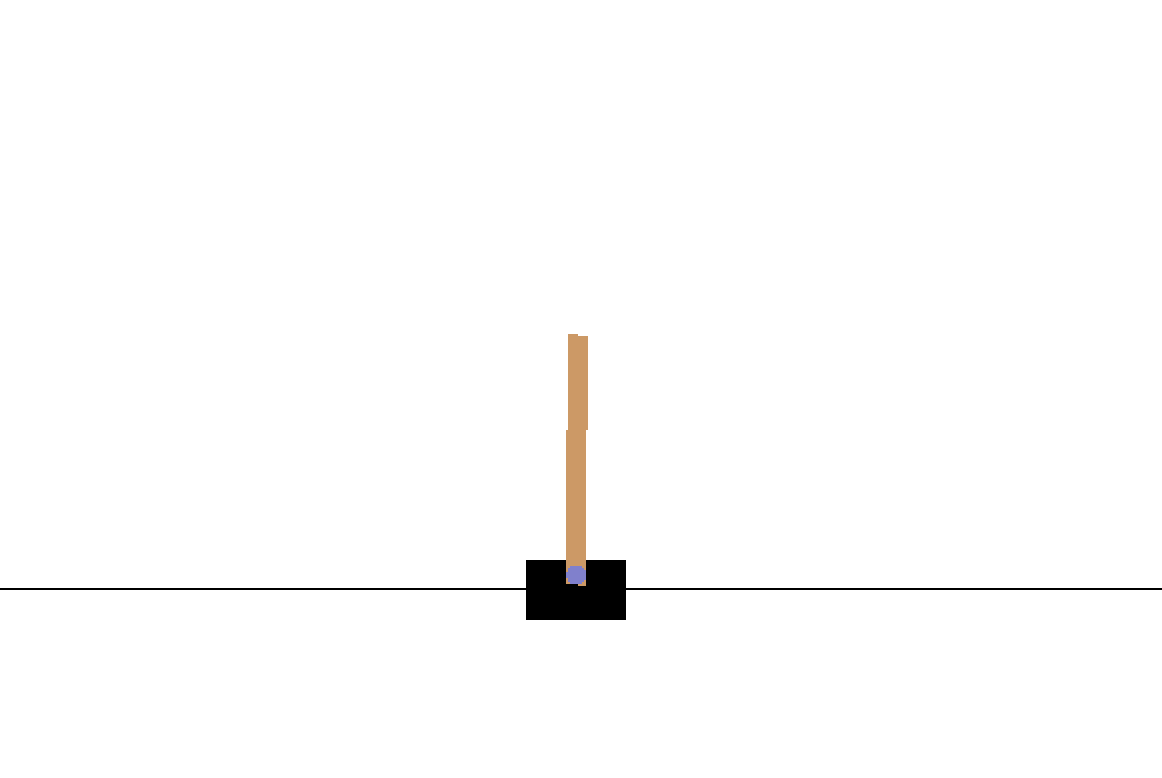
\includegraphics[scale=0.5]{include/cartpole.png}
    \caption{How the CartPole enviroment looks like}
    \label{fig:layers}
\end{figure}

In the CartPole environment a state consists of four elements: The position of cart and its velocity of cart aswell as the angle and the angular velocity of pole. In the CartPole problem we achieve a reward of +1 for every action performed that does not end the game. The only available actions are moving left and right.


\subsection{Atari 2600}

The Atari 2600 we will be using in this project, 



We are also using the Atari environment, here are some example of what these look like,

the action space, reward and done signals for the Atari environments are all pretty similar to what we saw with the CartPole enviroment, but the observation space in the Atari environments is an RGB image of the screen, which is an 3D matrix with shape (210, 160, 3) where every entry is the pixel value,



\begin{figure}[H]
    \begin{subfigure}[b]{.5\textwidth}
        \centering
        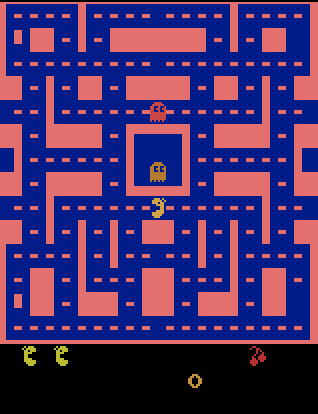
\includegraphics[scale=0.75]{include/pacman.png}
        \caption{Pacman environment}
    \end{subfigure}
    \begin{subfigure}[b]{.5\textwidth}
        \centering
        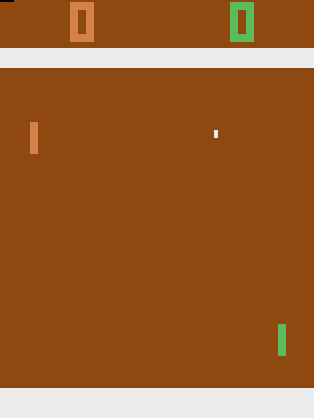
\includegraphics[scale=0.75]{include/pong.png}
        \caption{Pong environment}
    \end{subfigure}
    \vskip\baselineskip
    \begin{subfigure}[b]{.5\textwidth}
        \centering
        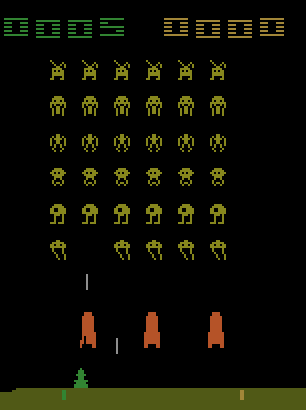
\includegraphics[scale=0.75]{include/space.png}
        \caption{Space invaders environment}
    \end{subfigure}
    \begin{subfigure}[b]{.5\textwidth}
        \centering
        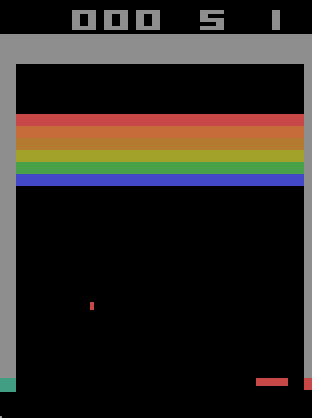
\includegraphics[scale=0.75]{include/breakout.png}
        \caption{Breakout environment}
    \end{subfigure}
    \caption{Four Atari environments}
    \label{fig:Atari_env}
\end{figure}
\end{document}
